\section{Задание 4. Приложение Рядов. Сиразетдинов Азат. Вариант 28}
\subsection{Задание 1}
Вычислить приближенно значение функции $ \cos48\degree $ с точностью 0,0001
\begin{flalign*} 
	\text{Возьмем табличное разложение}& &&\\
	&\cos x =  \sum_{k=0}^{\infty} (-1)^k \frac{x^{2k}}{(2k)!}&&\\
	&\cos48\degree = \cos(0,8378)&&\\
	\text{1 член последовательности:}& &&\\
	&\frac{0,8378^0}{1!} \approx 1&&\\
	\text{2 член последовательности:}& &&\\
	&(-1) * \frac{0,8378^2}{2!} \approx -0,35095&&\\
	\text{3 член последовательности:}& &&\\
	&\frac{0,8378^4}{4!} \approx 0,02052&&\\
	\text{4 член последовательности:}& &&\\
	&(-1) * \frac{0,8378^6}{6!} \approx -0,00048&&\\
	\text{4 член последовательности:}& &&\\
	&\frac{0,8378^8}{8!} \approx 0&&\\
	\text{Дальнейшие члены не будут изменять точность}& &&\\
	\cos(0,8378) \approx 1 - 0,35095 &+ 0,02052 - 0,00048 \approx 0,66909 \approx 0,6691&&\\
\end{flalign*}
Проверка:
\begin{center}
	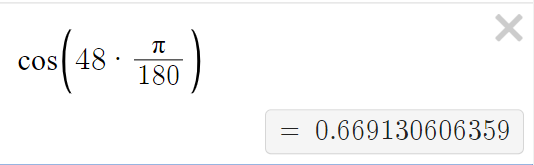
\includegraphics[width=.3\linewidth]{rgr2_task4_azat/cos_proof}\quad
\end{center}

\subsection{Задание 2}
Разлагая подынтегральную функцию в степенной ряд вычислить приближенно интеграл с точностью 0,0001\\
\begin{equation*}
	\int_0^{\frac{1}{2}} \frac{\ln(1+x^5)}{x^3} dx
\end{equation*}
\begin{flalign*} 
	&\text{Возьмем табличное разложение}&&\\
	&\int_0^{\frac{1}{2}} \frac{\ln(1+x^5)}{x^3} dx = 
	\int_0^{\frac{1}{2}} \frac{ \sum_{n=1}^\infty \frac{(-1)^{n-1} x^{5n}}{n} }{x^3} dx =
	\int_0^{\frac{1}{2}} \sum_{n=1}^\infty \frac{(-1)^{n-1}x^{5n}}{nx^3} dx =
	\sum_{n=1}^\infty \int_0^{\frac{1}{2}} \frac{(-1)^{n-1}x^{5n-3}}{n} dx = &&\\
	&=\sum_{n=1}^\infty \frac{(-1)^{n-1}x^{5n-2}}{n(5n-2)} \bigg|_0^{\frac{1}{2}} = 
	\sum_{n=1}^\infty \frac{(-1)^{n-1}}{n2^{5n-2}(5n-2)} &&\\
\end{flalign*}
\newpage
Подсчитаем первые члены последовательности:
\begin{flalign*} 
	\text{1 член последовательности:}& &&\\
	&\frac{1}{2^{3}*3} \approx 0,04167&&\\
	\text{2 член последовательности:}& &&\\
	&\frac{-1}{2*2^{8}*8} \approx -0,00024&&\\
	\text{3 член последовательности:}& &&\\
	&\frac{1}{3*2^{13}*13} \approx 0&&\\
	\text{Дальнейшие члены не будут изменять точность}& &&\\
	\int_0^{\frac{1}{2}} \frac{\ln(1+x^5)}{x^3} \approx 0,04167 &- 0,00024 = 0,04143 \approx 0,0414
\end{flalign*}
Проверка:
\begin{center}
	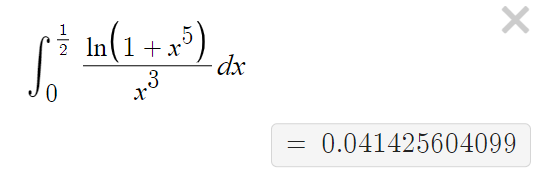
\includegraphics[width=.3\linewidth]{rgr2_task4_azat/int_proof}\quad
\end{center}

\subsection{Задание 3}
Найти в виде степенного ряда решение дифференциального уравнения,
удовлетворяющего заданным начальным условиям. Ограничиться четырьмя
членами ряда.
\begin{flalign*}
	&y'' = xy'- \ln y \\
	&y(2) = 1 \\
	&y'(2) = -1 \\
\end{flalign*}
\begin{flalign*}
	\text{Решение в виде ряда Тейлора: }& &&\\
	&y(x) = y(2) + y'(2)(x-2) + \frac{y''(2)(x-2)^2}{2!} + \frac{y'''(2)(x-2)^3}{3!}&&\\
	1) \ &y'' = xy' - \ln y &&\\
	&y''(2) = 2y'(2) - \ln y(2) = 2(-1) - \ln1 = -2 &&\\
	2) \ &y''' = (xy' - \ln y)' = y' + xy'' - \frac{1}{y} &&\\
	&y'''(2) = y'(2) + 2y''(2) - \frac{1}{y(2)} = -1 + 2(-2) - 1 = -4 &&\\
	\text{Подставим значения в ряд: }& &&\\
	&y(x) = y(2) + y'(2)(x-2) + \frac{y''(2)(x-2)^2}{2!} + \frac{y'''(2)(x-2)^3}{3!} = &&\\
	&=1 - (x-2) + \frac{-2 (x-2)^2}{2} + \frac{-4(x-2)^3}{6} =&&\\
	&= 1 - (x-2) - (x-2)^2 - \frac{2(x-2)^3}{3}&&\\
\end{flalign*}







